\documentclass[a4paper,12pt]{article}


% % % % % % % % % % % % % % % % % % % % % % % % % % % % %
% % ATTENTION : dans les figures le label doit être mis 
%APRES le caption pour que le numéro de la figure lorqu'on
%la référence soit le bon ; sinon on a le numéro du paragraphe
% % % % % % % % % % % % % % % % % % % % % % % % % % % % %

% package qui fournit \justify 
\usepackage[document]{ragged2e}

%pifont pour les puces de formes spéciales
\usepackage{pifont}
%\usepackage{svg}
% césure exemple
% \hyphenation{an-ti-cons-ti-tu-tion-nel

\usepackage[utf8x]{inputenc}
\usepackage[T1]{fontenc}
\usepackage[frenchb]{babel} % If you write in French
%\usepackage[english]{babel} % If you write in English
\usepackage{lmodern} % Pour changer le pack de police
\renewcommand*\familydefault{\sfdefault}
\usepackage{makeidx}
\usepackage{amsthm}
\usepackage{amsmath}
\usepackage{amssymb}
\usepackage{mathrsfs}
\usepackage{stmaryrd}
\usepackage{geometry}
%\usepackage{graphicx}
\usepackage{graphbox}
\usepackage{supertabular}
\usepackage{tabularx}
\usepackage{longtable}
\usepackage{pdflscape}
\geometry{hmargin=2cm,vmargin=2cm}

\usepackage{booktabs}
\usepackage{tabularx}
\usepackage[table]{xcolor}
\usepackage{ltablex}
\usepackage{float}
\usepackage{url}

\usepackage{chngcntr}
\counterwithin*{footnote}{page}


\usepackage[titletoc,toc,title,page]{appendix}
\renewcommand{\appendixtocname}{Annexes}
\renewcommand{\appendixpagename}{Annexes}

\usepackage{standalone}
\usepackage{ifthen}
\usepackage{xstring}
\usepackage{calc}
\usepackage{pgfopts}
\usepackage{tikz}
\usetikzlibrary{positioning,shapes,shadows,arrows}

\usepackage{algpseudocode}
\usepackage{algorithm}
\makeatletter
\renewcommand{\ALG@name}{Algorithme}
\renewcommand{\listalgorithmname}{Table des algorithmes}

\newtheorem{theo}{Définition}[section]
\usepackage{mathtools, bm}
\usepackage{amssymb, bm}

\usepackage{hyperref}
\hypersetup{
    colorlinks=true,       % false: boxed links; true: colored links
    linkcolor=black,       % color of internal links
    citecolor=purple,       % color of links to bibliography
    urlcolor=blue          % color of external links
}

\usepackage{listings}

\definecolor{dkgreen}{rgb}{0,.6,0}
\definecolor{dkblue}{rgb}{0,0,.6}
\definecolor{dkyellow}{cmyk}{0,0,.8,.3}

\lstset{
  language        = php,
  basicstyle      = \small\ttfamily,
  keywordstyle    = \color{dkblue},
  stringstyle     = \color{red},
  identifierstyle = \color{dkgreen},
  commentstyle    = \color{gray},
  emph            =[1]{php},
  emphstyle       =[1]\color{black},
  emph            =[2]{if,and,or,else},
  emphstyle       =[2]\color{dkyellow}}



\usepackage{blindtext}
\usepackage{enumitem} % pour changer les puces dans \itemize


\date{\today}

\makeindex
\def\siecle#1{\textsc{\romannumeral #1}\textsuperscript{e}}
\newcommand{\argmax}{\mathop{\mathrm{argmax}}\nolimits}
\newcommand{\pgcd}{\mathop{\mathrm{pgcd}}\nolimits}

\makeatletter
\renewcommand{\pod}[1]{\allowbreak\mathchoice
  {\if@display \mkern 18mu\else \mkern 8mu\fi (#1)}
  {\if@display \mkern 18mu\else \mkern 8mu\fi (#1)}
  {\mkern4mu(#1)}
  {\mkern4mu(#1)}
}

\usepackage{wallpaper}

\begin{document}
\renewcommand{\labelitemi}{\textbullet}
% pour factoriser l'échelle des figures 
%utilisation scale=\scaledvwa au lieu de scale = 0.3 ... 
\newcommand{\scaledvwa}{0.4} 
\newcommand{\scaledvw}{0.3}
\newcommand{\scalekad}{0.45}

\input{page-de-couverture/couv.tex}%on créé la couverture

\pagebreak

\tableofcontents
\justify

\pagebreak

\section*{Introduction}
\addcontentsline{toc}{section}{Introduction}



L'exercice proposé\footnote{Les livrables associés à cet exercice se trouvent à l'adresse : 
	\url{https://github.com/kad15/AF/tree/master/LIVRABLES_ATC_YUAN_BELDJILALI}} a pour finalité la modélisation et l'analyse d'un système ATC simplifié dans un cadre MBSE : Model Based System Engineering. Cette approche permet, en effet, des simulations et vérifications précoces intervenant lors de la phase décroissante du cycle en V, en amont de l'implémentation.   

\begin{figure}[H]
	\begin{center}	
		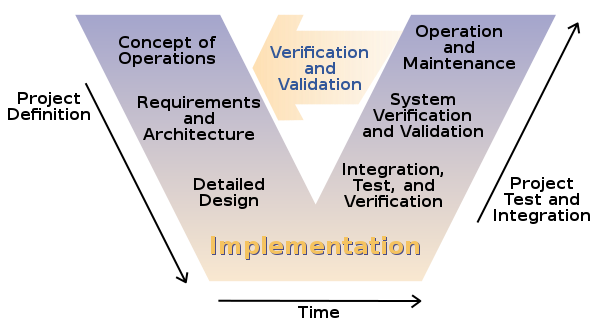
\includegraphics[scale=0.50]{images/v.png}
		\caption{Cycle en V}
		\label{v}
	\end{center}
\end{figure}

\paragraph{}
Les composants internes, constitutifs du système ATC considéré, comportent des acteurs humains, les contrôleurs, et des acteurs système, hardware et software. On citera, de façon non exhaustive, les radars primaires, secondaires, les logiciels de traitement et d'affichage des données radar et de plans de vol, sans oublier les filets de sauvegarde, les réseaux informatiques, les routeurs. Le NMOC européen, Network Management Operation Centre, et le système de traitement de plan de vol national sont inclus dans le système étudié car ils participent à la fourniture du service de contrôle. Par contre, les composants humains, matériels et logiciel assurant notamment le maintien en conditions opérationnelles des composants ne sont pas pris en compte dans le cadre de cet exercice.
\paragraph{}
Quant aux acteurs extérieurs, ce sont en particulier les pilotes, les compagnies aériennes, les aéronefs, le service météo. On pourrait ajouter les acteurs humains impactant la sûreté et la sécurité du système directement par le hacking du réseau ATC ou par brouillage des communications radio, par détournement de vols. Ceci impacte sur les contraintes que le système est susceptible de subir, contraintes qui doivent être prises en compte dans des fonctions additionnelles propres à empêcher les conséquences de malveillances et erreurs humaines et système. On peut aussi citer l'acteur environnemental "phénomènes météo". On choisit cependant de les ignorer pour se focaliser sur l'objectif pédagogique principal de cet exercice qui est d'appliquer une démarche MBSE sur un modèle simplifié.










\section{Pré-étude}


\subsection{ Diagramme de contexte }

Le système ATC étudié ici interagit avec quatre acteurs externes qui permettent de définir la frontière du système : 

\begin{itemize}
	\item Les compagnies aériennes,
	\item Les pilotes,
	\item Les aéronefs,
	\item Le service météo. 
\end{itemize}

Les acteurs environnementaux n'ont pas été pris en compte. La référence GPS de synchronisation est considérée comme appartenant au système

	\begin{figure}[H]
	\begin{center}	
		\includegraphics[scale=0.35]{images/ctx}
		\caption{Diagramme de contexte du système ATC}
		\label{ctx}
	\end{center}
\end{figure}

\subsection{ Description graphique du méta-modèle }

Les fonctions, les items et les composants sont les principaux éléments du méta modèle de la  figure \ref{meta}. En particulier, une fonction peut recevoir en entrée, ou fournir en sortie, un item information ou être déclenchée par un item signal électrique. La classe Requirement est intéressante dans le sens où elle permet de vérifier que les exigences sont toutes "mapées" avec un fonction qu'elle spécifie. 

\begin{figure}[H]
	\begin{center}	
\includegraphics[scale=0.50]{images/meta_modele}
\caption{meta modèle Vitech core conçu avec une version d'évaluation de l'outil Enterprise Architect}
\label{meta}
	\end{center}
\end{figure}


\subsection{ Données manipulées }

Les données manipulées sont les suivantes :
\begin{itemize}
	\item L'identifiant issu du plan de vol ou d'un radar secondaire,
	\item La position de l'aéronef.
\end{itemize}

La position d'un aéronef vu par un radar primaire ne donne que la distance et l'azimut. Les radars secondaires donnent en outre l'altitude et l'identifiant de l'appareil. Les positions radar doivent être converties en longitude/latitude WGS84 pour pouvoir être affichées. Ce dernier point n'a pas été pris en compte explicitement dans le modèle. En outre, le modèle CORE
ne distingue pas clairement entre position 2D des radars primaires et 3D des radars secondaires ; les fonctions de traitements spécifiques, ainsi que d'autres fonctions, ont été supprimées pour limiter la taille des  graphes hiérarchiques et EFFBD. Ceci constitue un écart par rapport au cahier des charges de l'énoncé mais reste dans l'esprit de l'exercice.

\section{Aspect fonctionnelle}
	
	\subsection{Décomposition fonctionnelle}
	
	L'analyse du sujet a conduit à quatre fonctions principales décomposées en sous-fonctions selon le diagramme hiérarchique de la figure \ref{hier} :
	
	\begin{itemize}
		\item Acquérir les informations, 
		\item Traiter les informations,
		\item Afficher les informations,
		\item Communiquer i.e. Echanger des informations
	\end{itemize}

L'analyse du modèle a mis en évidence, s'il en était besoin, le rôle crucial
de la communication entre contrôleur et pilote dans la fourniture du service de contrôle, d'alerte et de surveillance. Sur le plan métier, la radio comme moyen de communication constitue le maillon faible des systèmes ATC actuel. En ce sens, la modélisation permet 
de mettre en évidence des failles du domaine réel ce qui constitue une source d'amélioration du système. 
	
	\begin{figure}[H]
		\begin{center}	
			\includegraphics[scale=0.85]{images/hierarchique}
			\caption{Diagramme hiérarchique des fonctions}
			\label{hier}
		\end{center}
	\end{figure}
	
	\subsection{Scénario fonctionnel}

    Les diagrammes d'activités, EFFBD ou de séquence permettent de capturer un ou plusieurs scenarii du système modélisé. La démarche utilisée a consisté à créé un diagramme EFFBD dans CORE en utilisant uniquement les fonctions feuille puis de travailler sur le diagramme N2 pour l'ajout des items. Un exemple est donné en figure \ref{atc}.
    
    	\begin{figure}[H]
    	\begin{center}	
    		\includegraphics[scale=0.75]{images/atc}
    		\caption{Diagramme EFFBD simplifié du service ATC}
    		\label{atc}
    	\end{center}
    \end{figure}
    
    \paragraph{Scénario complet : }
     Le scénario associé à l'ensemble des fonctions feuille se trouve à l'adresse  \url{https://github.com/kad15/AF/blob/master/LIVRABLES_ATC_YUAN_BELDJILALI/question%207%20%20scenario%20fonctionnel%20unique.png}
    	

\section{Aspect produits }

\subsection{ Description graphique de la décomposition produit }
	\begin{figure}[H]
	\begin{center}	
		\includegraphics[scale=0.45]{images/atc_component}
		\caption{Diagramme entité-relation des composants du système ATC}
		\label{prod}
	\end{center}
\end{figure}

NB : Pour le tracé du diagramme ER, un composant conteneur abstrait atc\_component a été créé.


\begin{landscape}	
	\subsection{ Matrice de traçabilité Fonctions / composants }
	
	
	L'ensemble des fonctions vers l'ensemble des composants doit être une application surjective ; une fonction ne peut être assurée par deux composants différents dans le modèle Vitech core. Par contre, plusieurs composants peuvent effectuer la même fonction. La matrice de la figure \ref{fc} montre une couverture exhaustive des fonctions feuille par les composants du système. En particulier, la contrainte d'affichage sur un écran unique énoncée dans les spécifications est respectée.
	
	\begin{figure}[H]
		\begin{center}	
			\includegraphics[scale=0.65]{images/trace_fc}
			\caption{Matrice de traçabilité Fonctions / composants }
			\label{fc}
		\end{center}
	\end{figure}	

\end{landscape}


\subsection{ Matrice de traçabilité fonctions/input/output }
La matrice de traçabilité présentée dans les figures \ref{tfio} et \ref{tfio2} s'est avérée essentielle pour vérifier les entrées sorties des fonctions feuille.
En effet, malgré l'utilisation du diagramme N2, des oublis ont persisté ; seules les vues tabulaires permettent l'exhaustivité en mettant en évidence les manques. Ceci facilite l'approche récursive ou itérative propre à tout processus de conception ou développement. 

\paragraph{}
On regrettera le fait que les tables dans CORE ne puissent pas être directement générées au format \LaTeX.

\paragraph{}
Enfin, nous avons noté que le processus itératif se nourrit aussi des divergences potentielles entre l'ensemble des composants et celui des fonctions. On peut ainsi être amené à décomposer une fonction en sous fonctions ou un composant en sous composant. On arrive ainsi à une granularité optimale du FBS et du PBS  par "convergence des deux mondes".  

\begin{landscape}

\begin{figure}[H]
	\begin{center}	
		\includegraphics[scale=0.7]{images/tfio}
		
		\caption{Matrice de traçabilité Fonctions / in / out }
		\label{tfio}
	\end{center}
\end{figure}
	



	\begin{figure}[H]
		\begin{center}	
			\includegraphics[scale=0.7]{images/tfio2}
			\caption{Matrice de traçabilité Fonctions / in /out  (suite)}
			\label{tfio2}
		\end{center}
	\end{figure}
	
\end{landscape}

\section*{Conclusion}
\addcontentsline{toc}{section}{Conclusion}


\paragraph{}
La démarche employée est itérative. Dans l'approche MBSE, on divise le système en fonctions et sous fonctions, pour obtenir une structure d'arbre enraciné, que l'on confrontent d'un côté aux exigences et de l'autre aux composants qui assurent/perform ces fonctions. Le tracé de diagrammes dynamiques comme les EFFBD aident à visualiser le système en action, à décrire des scenarii, et donc à découvrir des fonctions qui auraient pu être oubliées et à régler le niveau de granuralité optimal au même titre que le reporting permis par CORE qui confronte functions, components, item et link dans une vue tabulaire efficace lors de la phase de détection des manques.  

\paragraph{}
Le reporting de CORE est aussi une aide précieuse pour la validation du projet en amont par le client et l'évaluation financière et ressources nécessaires à ce dernier. CORE est donc aussi un outil de communication convainquant.

\paragraph{}
Par manque de temps, les aspects "link" et "requirement" n'ont pu être traités pour aller au delà des objectifs de l'énoncé. Il manque probablement de plus à ce projet encore un certain nombre d'itérations. 

\paragraph{}
L'aspect Maintien en Conditions Opérationnelles(MCO) du système ATC n'a pas été abordé, celui du développement de ces systèmes non plus. En France, le MCO du système est assuré par les maintenances de la Direction des Opérations (DO) de la DGAC. Quant au développement, il relève de la Direction Technique et de l'Innovation(DTI) qui assure la MOA vis à vis des prestataires externes et le lien avec les partenaires, notamment dans le cadre de sa participation à certains "Work Package" du programme SESAR. En outre, comme indiqué dans l'introduction, nous avons choisi de faire abstraction des environnements "safety/security" et "phénomènes météo".   

\paragraph{}
Enfin, un dernier mot sur l'outil utilisé. CORE est un outil efficace pour aider à construire "the right system and the system right" mais trop lié au monde Windows. En particulier, une meilleure connaissance de l'outil auraient permis un gain de temps important dans le cadre du projet ROBAFIS bien que la version "university" n'autorise pas le travail collaboratif. CORE permet, en effet, d'assurer l'exhaustivité de la prise en compte des exigences par les fonctions et la création automatique des tableaux pour alimenter le rapport de développement Encore faut-il s'assurer que les exigences traduisent correctement les besoins.


%\newpage
%\appendix
%\include{annexes/annexe_A}
%\include{annexes/annexe_B}

\newpage
\nocite{*}  %affiche toutes les entrées du bib même celles qui ne sont pas citées.
% cf.    http://www.tuteurs.ens.fr/logiciels/latex/bibtex.html
% compilation en TROIS PHASE  bibtex traite un fichier *.aux mais bibtex mon_fichier comme bibtex mon_fichier.aux sont acceptés 
% latex mon_fichier.tex
% bibtex mon_fichier
% latex mon_fichier.tex


% \renewcommand{\bibname}{Toto}
% ou
%\renewcommand{\refname}{Bibliographie}
% dans le préambule.
%\bibliographystyle{alpha}
%\bibliography{references}
\input{page-de-couverture/page_blanche}
\input{page-de-couverture/quatrieme-de-couv}
\end{document}
